
\chapter{CNN (Coursera)}


\section{Convolutional Neural Networks}
\section{Convolutional layer}


Input tensor:
\begin{equation}
    n_H^{l-1} \times n_W^{l-1} \times n_c^{l-1}
\end{equation}

Output tensor:
\begin{equation}
    n_H^l \times n_W^l \times n_c^l
\end{equation}

The \textbf{convolutional filter} at layer $l$ has size: $f^l \times f^l \times n_c^{l-1}$ It has always the same number of channels as the input tensor. So the result after one convolutional filter is a "flat image" of size $n_H^l \times n_W^l \times 1$. Usually, a convolutional layer has $n_c^l$ filters and all the results are stacked.

After a convolution the size becomes:

\begin{equation}
    n_H^l = \left\lfloor \frac{n_H^{l-1} + 2 p^l - f^l}{s^l} + 1 \right\rfloor
\end{equation}
\begin{equation}
    n_W^l = \left\lfloor \frac{n_W^{l-1} + 2 p^l - f^l}{s^l} + 1 \right\rfloor
\end{equation}

where $p^l$ is the padding, $f^l$ is the filter size (usually an odd number) and $s^l$ is the stride.


When we use \textbf{vectorized operations}, for example with mini-batches, we add a dimension at the beginning:
\begin{equation}
    m \times n_H^l \times n_W^l \times n_c^l
\end{equation}


Each convolutional filter also have a \textbf{bias}, a single number that is added on each pixel of the resulting "flat image". Thus, the full layer has $n_c^l$ biases, usually written $1 \times 1 \times n_c^l$.

\section{Pooling layer}

A pooling layer has no weights, but only hyper-parameters:
\begin{itemize}
    \item filter size $f$
    \item stride $s$
    \item max or average pooling
\end{itemize}
Note that usually there is no padding on pooling layers.

The same formula as for convolution can be used to compute the output size:
\begin{equation}
    n_H^l = \left\lfloor \frac{n_H^{l-1} - f^l}{s^l} + 1 \right\rfloor
\end{equation}
\begin{equation}
    n_W^l = \left\lfloor \frac{n_W^{l-1} - f^l}{s^l} + 1 \right\rfloor
\end{equation}
\begin{itemize}
    \item A pooling layer does not change the \textbf{number of channels}. It is applied on each layer separately.
    \item A typical size is $f=2$, $s=2$ which has the effect of dividing the width and height by 2. 
    \item The idea for \textbf{max pooling} is: if a feature is detected in a region (a high value in the feature map), keep this high value.
    \item The \textbf{average pooling} is more rare. It can be used at the end to pass from $h\times w \times n$ to $1 \times 1 \times n$.
\end{itemize}



\section{Fully connected Layer}
A fully connected layer (\textbf{FC}) is defined by:
\begin{equation}
    \begin{split}
        &z^i = W^i a^{i-1} + b^i \\
        &a^i = g(z^i)
    \end{split}
\end{equation}

\section{Neural network}
\begin{itemize}
    \item Usually a \textbf{convolutional layer + a pooling layer} count as 1 layer, as the pooling layer has no trainable weights.
    \item A \textbf{common pattern} is to alternate: some conv - pool - some conv - FC - FC - FC - softmax

\end{itemize}




\section{Why convolutions}
\begin{itemize}
    \item \textbf{Parameter sharing:} A feature detector (for example vertical edges detector) that is useful in one part of the image can is probably also useful in an other part. With convolutions the filter can be re-used everywhere in the image.
    \item \textbf{Sparsity of connections:} In each layer, each output value depends only on a small numbers of of inputs.
    \item \textbf{Invariance to translation:} This is implied by convolution. The same image of a cat just translated will give very similar features.
\end{itemize}


\section{Deep networks}
\begin{itemize}
    \item Deeper networks are able to fit more complex function
    \item Making a network deeper does not always help because it make the training more complex.
\end{itemize}

\section{ResNet}
\begin{itemize}
    \item Skip connections make it very easy to learn the identity function. This means that adding a residual block doesn't harm the training of the network.
    \item Skip connections help to avoid vanishing gradient
\end{itemize}

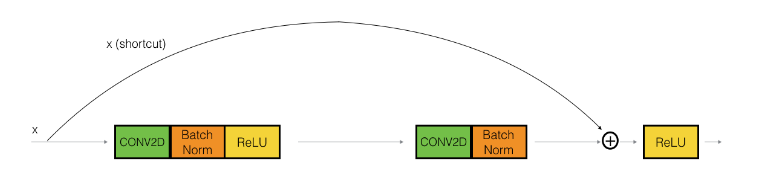
\includegraphics[scale=0.25]{content/resnet_block.png}



\section{Technique to gain performance}
\begin{itemize}
    \item Ensembling: you train several networks for the same task and average the last layers
    \item Multiple crop at test time: crop several sub-image from the test image, run the network and average the results.
\end{itemize}

\section{Dimensionality Reduction}
\subsection{PCA}
The idea of PCA is to build $n\_e$ new independent features that are \textbf{linear combinations} of the $n\_d$ old features, so that the projections of the data on this new subspace are as close as possible to the initial data. In other words, \textbf{PCA is looking for the best linear subspace of the initial space} (described by an orthogonal basis of new features) such that the error of approximating the data by their projections on this subspace is as small as possible.
This can be obtained using the \textbf{eigenvector decomposition}, by keeping the $n\_e$ eigen vectors associated with the largest eigen values.

\subsection{Auto-Encoder}
\begin{itemize}
    \item With Auto-Encoders with are looking for the best encoder and decoder that \textbf{keeps the maximum of information}. With neural networks this is achieved with an iterative optimization.
    \item If we suppose we have a \textbf{linear auto-encoder} (both the encoder and the decoder has only one linear layer, without non-linearity), this is \textbf{very close to PCA}. Several bases can be chosen to describe the same optimal subspace. PCA selects the one that maximizes the variances of the data along the first dimension and the basis is orthogonal. With neural networks there is not this orthogonality constraint. Thus, the found basis may be different.
    \item Traditional auto-encoders are \textbf{deep and non-linear}, such that they can proceed to high dimensionality reduction while keeping the reconstruction loss low.
    \item An encoder with "infinite power" could theoretically take N initial data points and reduce them as 1, 2, 3, ... up to N  and the associated decoder make the reverse transformation with no loss.
    \item Dimensionality reduction with no reconstruction loss often gives a \textbf{lack of interpretability and exploitable structures} in the latent space (\textbf{lack of regularity}.
    \item the final purpose of dimensionality reduction is not to only reduce the number of dimensions of the data but to reduce this number of dimensions \textbf{while keeping the major part of the data structure information} in the reduced representations.
    \item For these two reasons, the dimension of the latent space and the depth of auto-encoders (that define degree and quality of compression) have to be carefully controlled and adjusted depending on the final purpose of the dimensionality reduction.
\end{itemize}


\subsection{Generative model}
\begin{itemize}
    \item To have good generative properties, the latent space must be \textbf{regular} (well organized)
    \item Auto-encoders are trained to minimize the reconstruction error, \textbf{no matter how the latent space is organized}.
    \item Auto-encoders with high degrees of freedom can encoder and decode with no information loss, however this leads to \textbf{severe overfitting}, implying that some points of the latent space will give meaningless content once decoded.
    \item Due to overfitting, the latent space of an auto-encoder can be extremely irregular (close points in latent space can give very different decoded data, some point of the latent space can give meaningless content once decoded, ...).
\end{itemize}

\subsection{Variational Auto-Encoder}
\begin{itemize}
    \item  It can be defined as being an auto-encoder whose training is \textbf{regularised} to avoid overfitting and ensure that the latent space has \textbf{good properties} that enable generative process.
    \item Instead of encoding an input as a single point, we encode it as a \textbf{distribution} over the latent space.
    \item Its loss is composed of a \textbf{reconstruction term} (on the final layer) and a \textbf{regularisation term} (on the latent space).
    \item That regularisation term is expressed with the \textbf{Kullback-Leibler divergence} between the returned distribution and a standard Gaussian distribution.
    \item The \textbf{regularity} expected from the latent space can be expressed through two main properties:
    \begin{itemize}
        \item \textbf{continuity}: two close points in the latent space should give similar contents once decoded (not totally different).
        \item \textbf{completeness}: for a chosen distribution, a points sampled from the latent space should give "meaniningfull" content once decoded.
    \end{itemize}
    \item The regularization term should avoid to have punctual distributions (tiny variances) or very different means. 
    
    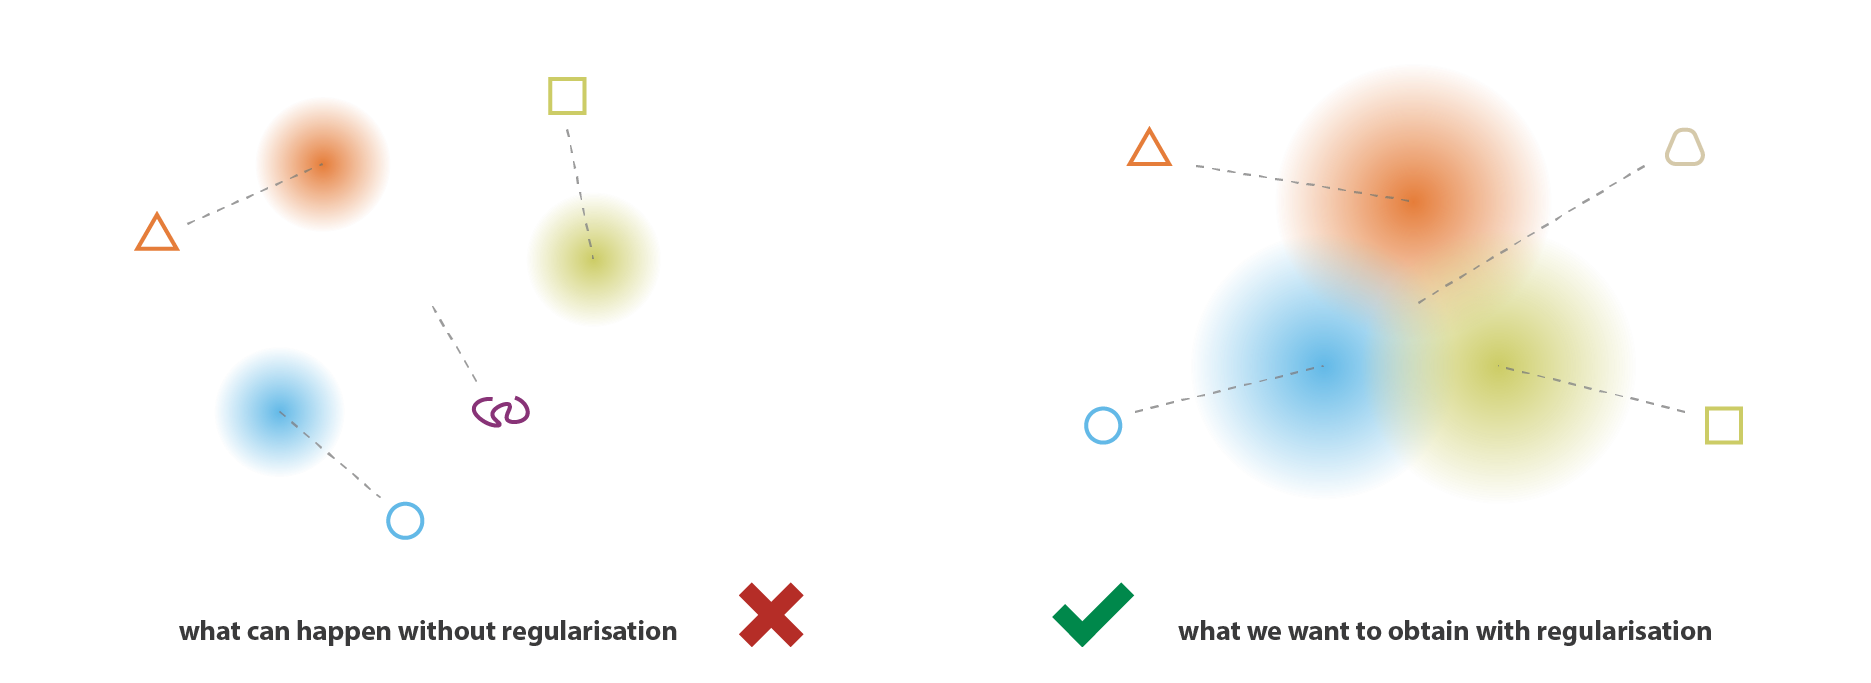
\includegraphics[scale=0.2]{content/latent_space_regularisation.png}

    \item The encoder is composed of two functions $g$ and $h$, that share the first layers and predict respectively the \textbf{mean} and \textbf{variances}.
    \item The covariance matrix of the latent space distribution is assumed to be diagonal for simplicity.
    \item The loss equation can be derived using a probabilistic approach and \textbf{variational inference}.
    \item The \textbf{reparametrisation trick} is used ot make gradient descent possible despite the random sampling, using the fact that a distribution $\mathcal{N}(g, H)$ can be written as $z=h(x)M+g(x)$ with $M\sim\mathcal{N}(0, I)$.

    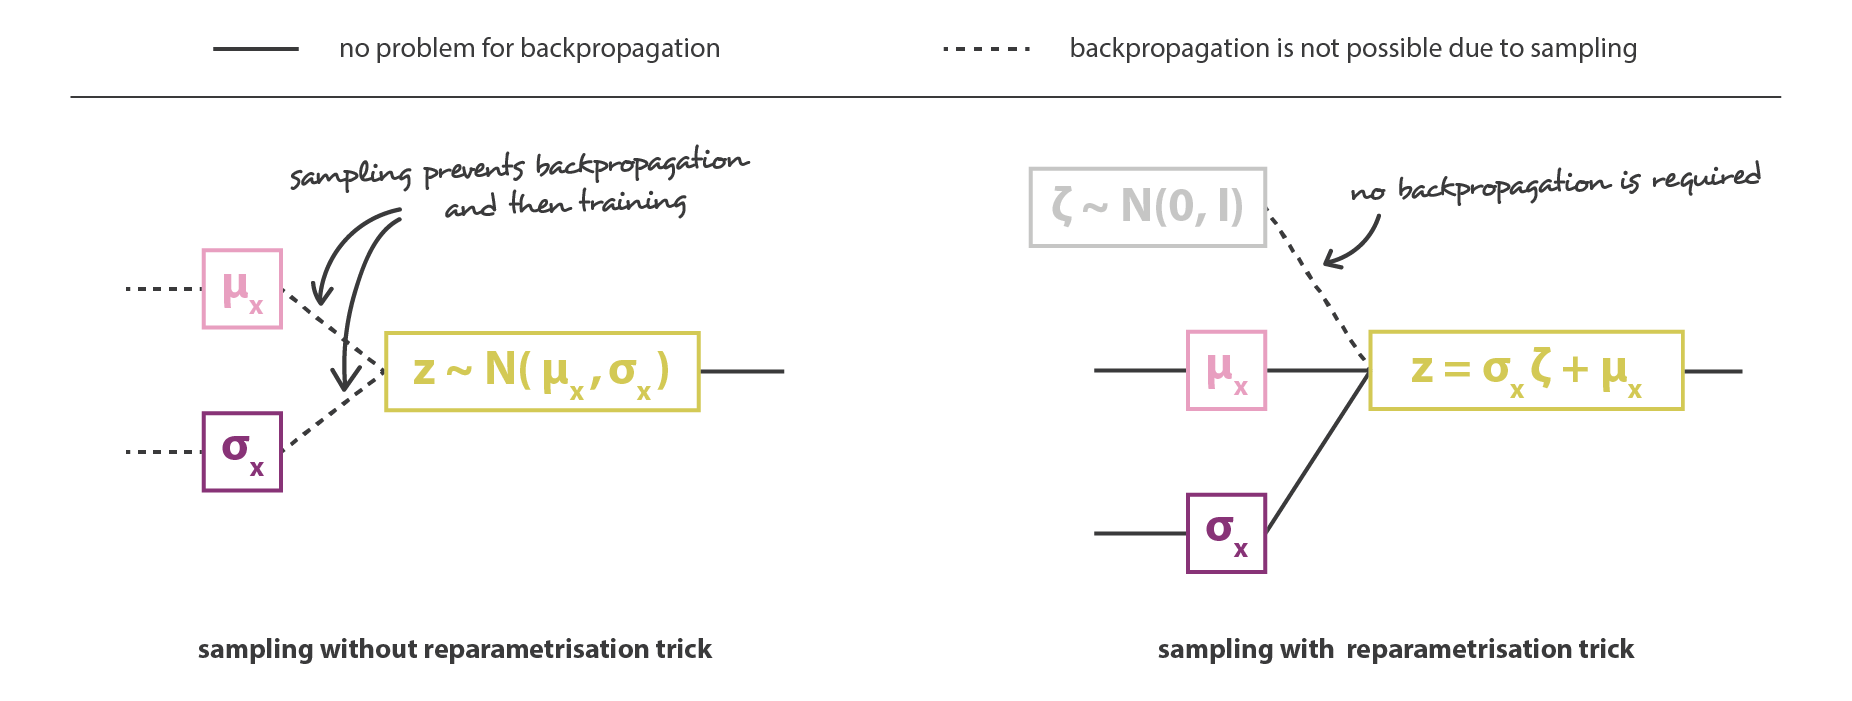
\includegraphics[scale=0.2]{content/reparametrisation_trick.png}
    
    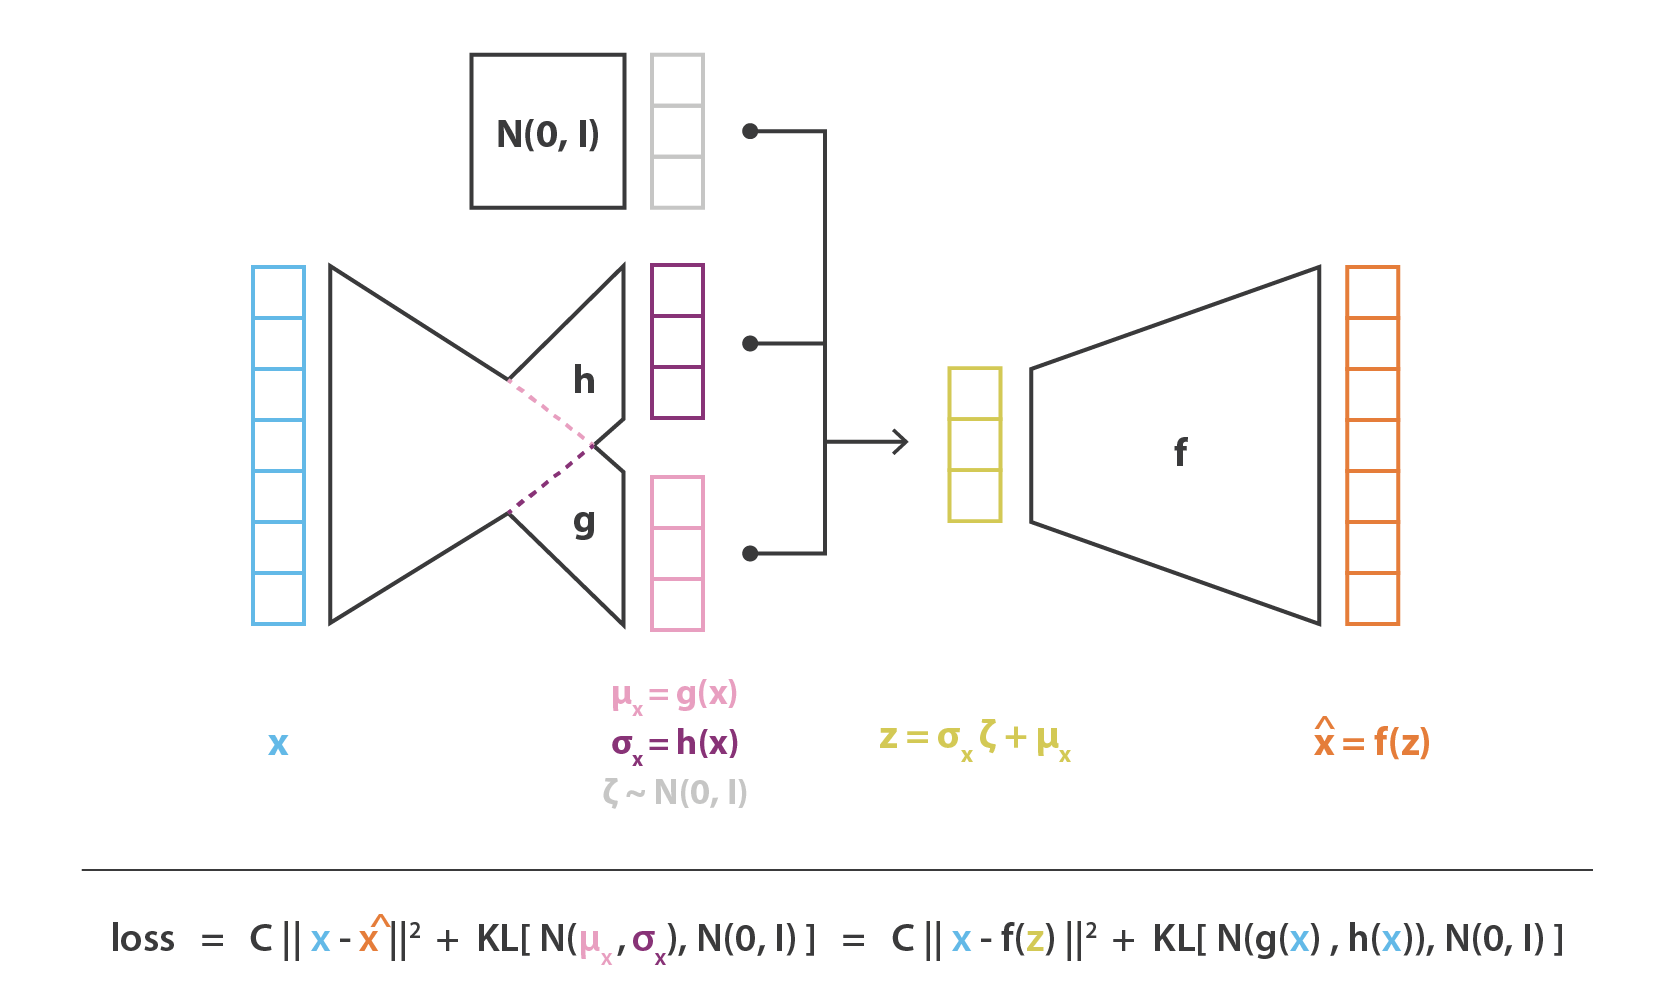
\includegraphics[scale=0.2]{content/final_vae_architecture.png}

\end{itemize}
\subsection{Conclusion}
\href{https://towardsdatascience.com/understanding-variational-autoencoders-vaes-f70510919f73}{https://towardsdatascience.com/understanding-variational-autoencoders-vaes-f70510919f73}

Due to overfitting, the latent space of an auto-encoder can be extremely irregular (close points in latent space can give very different decoded data, some point of the latent space can give meaningless content once decoded, ...). That's why VAE are needed.
However, GANs are more used, maybe because of their lower complexity compared to VAEs (probabilistic models + variational inference).


\subsection{Mathematical derivation of KL in VAEs}

The encoder distribution is $q(z|x) = \mathcal{N}(z|\mu(x),\Sigma(x))$, where $\Sigma=diag(\sigma_1^2, \sigma_2^2, ..., \sigma_n^2)$.
The latent prior is given by $p(z) = \mathcal{N}(0, I)$.
Both are multivariate Gaussian of dimensions $n$, for which the KL divergence is:
\begin{equation}
    \mathcal{D_{KL}}[p_1||p_2] = \frac{1}{2} \left[ \log \frac{|\Sigma_2|}{|\Sigma_1|} - n + Tr\{\Sigma_2^{-1}\Sigma_1\} + (\mu_2 - \mu_1)^T \Sigma_2^{-1} (\mu_2-\mu_1) \right]
\end{equation}

For VAEs, $\mu_1 = \mu$, $\mu_2 = 0$, $\Sigma_1 = \Sigma$, $\Sigma_2 = I$, which gives:
\begin{equation}
    \begin{split}
        \mathcal{D_{KL}}[q(z|x)||p(z)] &= \frac{1}{2} \left[ \log \frac{1}{|\Sigma|} - n + Tr\{I^{-1}\Sigma\} + (0 - \mu)^T I^{-1} (0-\mu) \right] \\
        &= \frac{1}{2} \left[ -\log |\Sigma| - n + Tr\{\Sigma\} + \mu^T\mu \right] \\
        &= \frac{1}{2} \left[ -\log \prod_i \sigma_i^2 - n + \sum_i \sigma_i^2 + \sum_i \mu_i^2 \right] \\
        &= \frac{1}{2} \left[ -\sum_i \log\sigma_i^2 - n + \sum_i \sigma_i^2 + \sum_i \mu_i^2 \right] \\
        \mathcal{D_{KL}}[q(z|x)||p(z)] &= \frac{1}{2} \left[ -\sum_i(\log\sigma_i^2 + 1) + \sum_i \sigma_i^2 + \sum_i \mu_i^2 \right] \\
    \end{split}
\end{equation}

This is simple to implement in PyTorch.

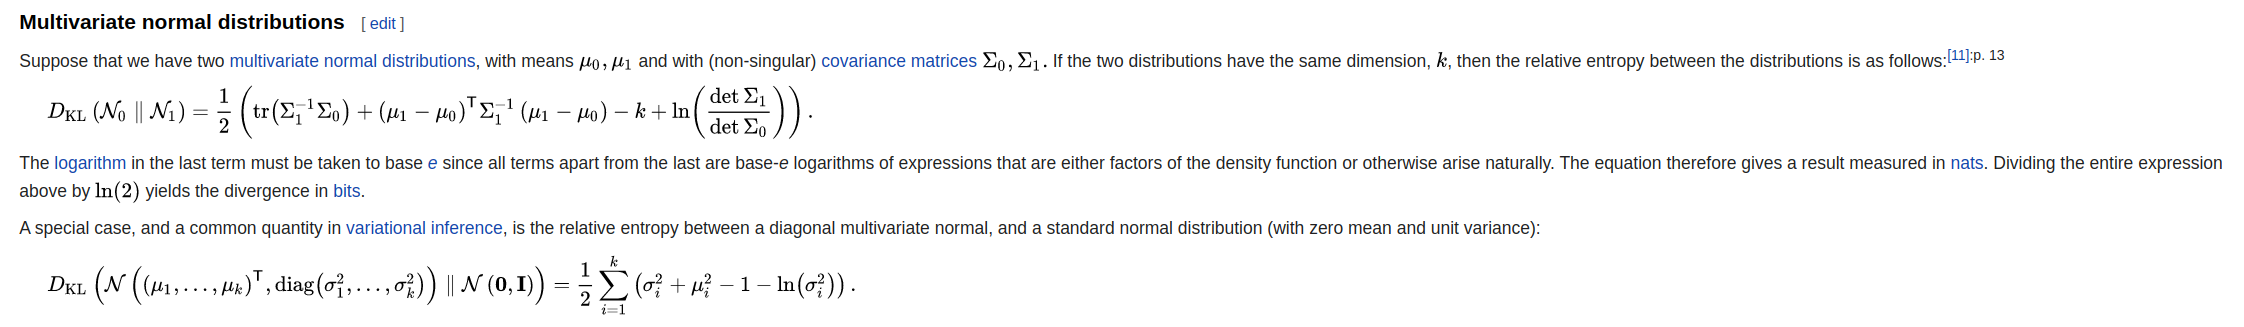
\includegraphics[scale=1]{content/KL_gaussians.png}
To get this equation, we should use the "trace trick" (see \href{https://en.wikipedia.org/wiki/Estimation_of_covariance_matrices#The_trace_of_a_1_.C3.97_1_matrix}{trick})